%% LyX 2.0.6 created this file.  For more info, see http://www.lyx.org/.
%% Do not edit unless you really know what you are doing.
\documentclass[english]{article}
\usepackage[T1]{fontenc}
\usepackage[utf8]{luainputenc}
\usepackage[a4paper]{geometry}
\geometry{verbose,tmargin=0.5in,bmargin=1in,lmargin=1in,rmargin=1in}
\usepackage{babel}
\usepackage{pdfpages}
\usepackage[unicode=true,pdfusetitle,
 bookmarks=true,bookmarksnumbered=true,bookmarksopen=true,bookmarksopenlevel=1,
 breaklinks=false,pdfborder={0 0 1},backref=false,colorlinks=false]
 {hyperref}

\makeatletter

%%%%%%%%%%%%%%%%%%%%%%%%%%%%%% LyX specific LaTeX commands.
%% A simple dot to overcome graphicx limitations
\newcommand{\lyxdot}{.}


%%%%%%%%%%%%%%%%%%%%%%%%%%%%%% User specified LaTeX commands.
\usepackage{pgfplots} 
\usepackage{tikz}
\usepackage{pst-node} 
\usetikzlibrary{fit,shapes}   
\usetikzlibrary{arrows}

\makeatother

\begin{document}
\includepdf{Assignment_Submission_and_Declaration_Form_2}\pagebreak{}


\title{124MS - Coursework 2}


\author{Vitor Morato Almeida}

\maketitle
\pagebreak{}
\begin{enumerate}
\item \textbf{The functions f : \{1, 2, 3\} → \{a, b\} and g : \{a, b\}
→ \{x, y, z\} are given by f(1) = b, f(2) = b, f(3) = a, g(a) = y,
g(b) = x. }

\begin{enumerate}
\item \textbf{Classify each of f and g as bijective, injective, surjective,
or neither. }\\
\textbf{}\\
Lets draw the mapping diagrams to help to classify each function\\
\textbf{}\\
\begin{center}
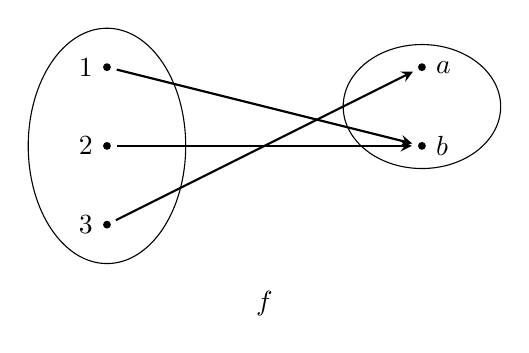
\begin{tikzpicture}[
	>=stealth,
	bullet/.style={
		fill=black,
    	circle,
    	minimum width=1pt,
		inner sep=1pt
	},     
	projection/.style={
		->,
		thick,
		shorten <=2pt,
		shorten >=2pt
	},
	every fit/.style={
		ellipse,
		draw,
		inner sep=0pt
	}
 ]

	\foreach \y/\l in {1/3,2/2,3/1}
		\node[bullet,label=left:$\l$] (a\y) at (0,\y) {};
	\foreach \y/\l in {2/b,3/a}
		\node[bullet,label=right:$\l$] (b\y) at (4,\y) {};
	
	\node[draw,fit=(a1) (a2) (a3),minimum width=2cm] {};
	\node[draw,fit=(b2) (b3),minimum width=2cm] {} ;
	
	\draw (2,0) node {$f$};

	
    \draw[projection] (a1) -- (b3);
	\draw[projection] (a2) -- (b2);
	\draw[projection] (a3) -- (b2);



\end{tikzpicture}
\end{center}from the diagram of function $f$ above we can see that every element
of the codomain is mapped to by at least one element of the domain,
so function $f$ is surjective\\
\begin{center}
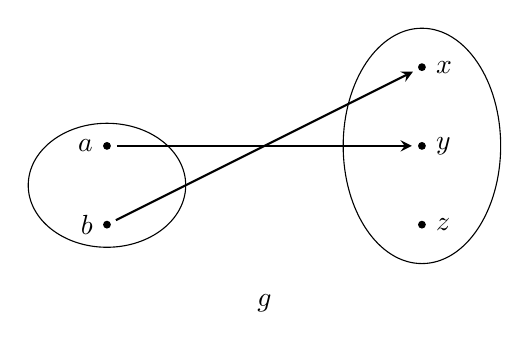
\begin{tikzpicture}[
	>=stealth,
	bullet/.style={
		fill=black,
    	circle,
    	minimum width=1pt,
		inner sep=1pt
	},     
	projection/.style={
		->,
		thick,
		shorten <=2pt,
		shorten >=2pt
	},
	every fit/.style={
		ellipse,
		draw,
		inner sep=0pt
	}
 ]

	\foreach \y/\l in {2/a,1/b}
		\node[bullet,label=left:$\l$] (a\y) at (0,\y) {};
	\foreach \y/\l in {3/x,2/y,1/z}
		\node[bullet,label=right:$\l$] (b\y) at (4,\y) {};
	
	\node[draw,fit=(a1) (a2),minimum width=2cm] {};
	\node[draw,fit=(b1) (b2) (b3),minimum width=2cm] {} ;
	
	\draw (2,0) node {$g$};

	
    \draw[projection] (a1) -- (b3);
	\draw[projection] (a2) -- (b2);




\end{tikzpicture}
\end{center}from the diagram of function $g$ above we can see that every element
of the codomain is mapped to by at most one element of the domain,
so function $g$ is injective\\
\\
As none of the functions above is simultaneously surjective and injective,
we can't classify them as bijective.\\

\item \textbf{Find $g\circ f$. }\\
\textbf{}\\
This time I'm going to use the previous diagrams to build the diagram
of the composition g ◦ f\textbf{ }\\
\textbf{}\\
\begin{center}
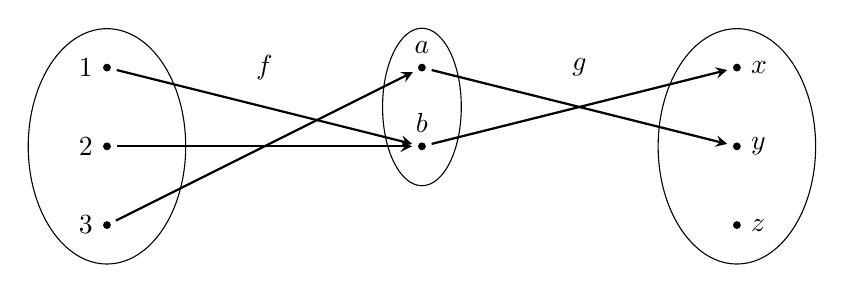
\begin{tikzpicture}[
	>=stealth,
	bullet/.style={
		fill=black,
    	circle,
    	minimum width=1pt,
		inner sep=1pt
	},     
	projection/.style={
		->,
		thick,
		shorten <=2pt,
		shorten >=2pt
	},
	every fit/.style={
		ellipse,
		draw,
		inner sep=0pt
	}
 ]

	\foreach \y/\l in {1/3,2/2,3/1}
		\node[bullet,label=left:$\l$] (a\y) at (0,\y) {};
	\foreach \y/\l in {2/b,3/a}
		\node[bullet,label=above:$\l$] (b\y) at (4,\y) {};
	\foreach \y/\l in {3/x,2/y,1/z}
		\node[bullet,label=right:$\l$] (c\y) at (8,\y) {};
	
	\node[draw,fit=(a1) (a2) (a3),minimum width=2cm] {};
	\node[draw,fit=(b2) (b3),minimum width=1cm,minimum height=2cm] {} ;
	\node[draw,fit=(c1) (c2) (c3),minimum width=2cm] {};
	
	\draw (2,3) node {$f$};
	\draw (6,3) node {$g$};

	
    \draw[projection] (a1) -- (b3);
	\draw[projection] (a2) -- (b2);
	\draw[projection] (a3) -- (b2);
	\draw[projection] (b2) -- (c3);
	\draw[projection] (b3) -- (c2);



\end{tikzpicture}
\end{center}Summarizing the diagram we have,\\
\begin{center}
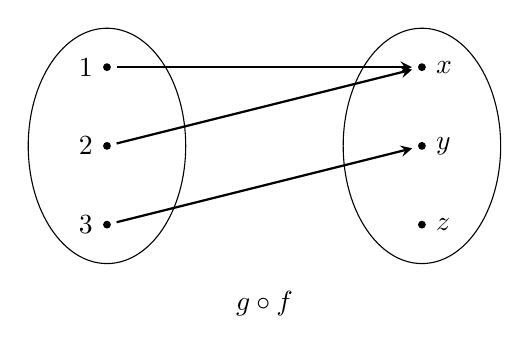
\begin{tikzpicture}[
	>=stealth,
	bullet/.style={
		fill=black,
    	circle,
    	minimum width=1pt,
		inner sep=1pt
	},     
	projection/.style={
		->,
		thick,
		shorten <=2pt,
		shorten >=2pt
	},
	every fit/.style={
		ellipse,
		draw,
		inner sep=0pt
	}
 ]

	\foreach \y/\l in {1/3,2/2,3/1}
		\node[bullet,label=left:$\l$] (a\y) at (0,\y) {};
	\foreach \y/\l in {3/x,2/y,1/z}
		\node[bullet,label=right:$\l$] (c\y) at (4,\y) {};
	
	\node[draw,fit=(a1) (a2) (a3),minimum width=2cm] {};
	\node[draw,fit=(c1) (c2) (c3),minimum width=2cm] {};
	
	\draw (2,0) node {$g \circ f$};

	\draw[projection] (a1) -- (c2);
	\draw[projection] (a2) -- (c3);
	\draw[projection] (a3) -- (c3);



\end{tikzpicture}
\end{center} 
\item \textbf{Either find the inverse of g ◦ f or explain why $g\circ f$
is not invertible}\\
\textbf{}\\
$g\circ f$ is not invertible because it cannot be classified as bijective.\\

\end{enumerate}
\item \textbf{I want to develop a database of information about my book
collection, which tells me about the authors and genres of the various
books I own. At the moment I have books by Isaac Asimov, China Mieville,
Peter F Hamilton and Arthur C Clarke, and I denote the set of authors
by A = \{A, M, H, C\}, abbreviating each author by the initial of
his surname. I am classifying the books as science fiction, fantasy,
horror and non-fiction, so my set of genres is G = \{s, f , h, n\},
again using initial letters as abbreviations. At the moment, I have
science fiction works by China Mieville and Isaac Asimov, I have fantasy
by Peter F Hamilton and China Mieville, horror by Peter F Hamilton
and Arthur C Clarke, and non-fiction by Isaac Asimov.}

\begin{enumerate}
\item \textbf{Give the relation R on A × G which represents this information.
(You may use appropriate abbreviations.) }\\
\\
$R=\{(A,s),(A,n),(M,s),(M,f)(H,f),(H,h),(C,h)\}$
\end{enumerate}
\item [3.]

\begin{enumerate}
\item \textbf{Draw the graph with adjacency matrix}\\
\begin{center} \textbf{A =$\left[\begin{array}{ccccc}
0 & 0 & 0 & 1 & 1\\
0 & 0 & 1 & 0 & 0\\
0 & 1 & 0 & 1 & 0\\
1 & 0 & 1 & 0 & 1\\
1 & 0 & 1 & 1 & 0
\end{array}\right]$ }\end{center}This the graph generated from adjacency matrix:\\
\begin{center}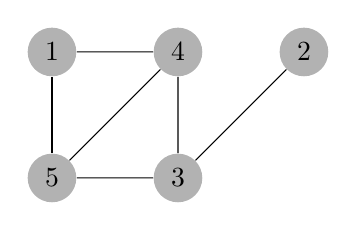
\begin{tikzpicture}[
		scale=.8,auto=left,
		every node/.style={circle,fill=gray!60}
		] 
	
	\node (n1) at (0,10) {1}; 
	\node (n2) at (4,10) {2};
	\node (n3) at (2,8) {3};
	\node (n4) at (2,10) {4};
	\node (n5) at (0,8) {5};

	\foreach \from/\to in {n1/n4, n1/n5,n2/n3, n3/n5, n3/n4, n4/n5} 
		\path (\from) edge (\to);

\end{tikzpicture}\end{center}
\item Calculate $A^{2}$ and hence find the number of paths of length 2 from
vertex 1 to vertex 5.\\
\\
\begin{eqnarray*}
A\times A & = & \left[\begin{array}{ccccc}
2 & 0 & 2 & 1 & 1\\
0 & 1 & 0 & 1 & 1\\
2 & 0 & 3 & 1 & 1\\
1 & 1 & 1 & 3 & 2\\
1 & 1 & 1 & 2 & 3
\end{array}\right]\\
\end{eqnarray*}
\\
Looking at the position (1,5), also (5,1) once this is not a directed
graph, we can see that there is only one path of length 2. 
\end{enumerate}
\item [7.]\textbf{Bob decides to use n = 221 = 13 × 17 and e = 11 as his
public key for an RSA cryptosystem. }

\begin{enumerate}
\item \textbf{Show that the decryption exponent is 35. }\\
\textbf{}\\
To show that 35 is a decryption exponent, we need to check the following
condition:\textbf{}\\
\textbf{}\\
$ed$ $\equiv$ $1$ (mod z)\textbf{}\\
\textbf{}\\
To calculate z we use the following formula:\\
\\
$z=(p-1)(q-1)$\\
\\
replacing the $p$ and $q$ values from question into the formula
we have:\\
\\
$z=(13-1)(17-1)=192$\\
\\
now we calculate $ed$ and its module of 192\\
\\
$ed=11\times35=385$\\
$385/192=2\frac{1}{192}\equiv1$ (mod z)\\

\item \textbf{Find the encrypted form of the message 16.}\\
\textbf{}\\
$C=M^{e}$ (mod n)\\
$C=16^{11}$(mod 221)\\
\\
$11=8+2+1$\\
\\
$16^{1}\equiv35$ (mod 221)\\
$16^{2}=256\equiv35$ (mod 221)\\
$16^{4}\equiv35^{2}=1225\equiv120$ (mod 221)\\
$16^{8}\equiv120^{2}=14400\equiv35$ (mod 221)\\
\\
$C=16^{8}\times16^{2}\times16\equiv35\times35\times16=19600\equiv152$
(mod 221)\end{enumerate}
\end{enumerate}

\end{document}
